\pagestyle{empty}
\cleardoublepage
\pagestyle{fancy}

\selectlanguage{english}


\chapter{Modularity: Genes, Development, and Evolution}\label{aree}

Diogo Melo*, Arthur Porto*, James Cheverud, Gabriel Marroig

\begin{verbatim}
*Contributed equally
Published in:
Annu. Rev. Ecol. Evol. Syst. 2016. 47:463-486
doi: 10.1146/annurev-ecolsys-121415-032409
Copyright © 2016 by Annual Reviews. All rights reserved
\end{verbatim}

\newpage

\vspace*{10pt}
% Abstract
\begin{center}
  \emph{\begin{large}Abstract\end{large}}
\vspace{2pt}
\end{center}

\noindent
Modularity has emerged as a central concept for evolutionary biology, thereby providing the field with a theory of organismal structure and variation. This theory has reframed long-standing questions and serves as a unified conceptual framework for genetics, developmental biology, and multivariate evolution. Research programs in systems biology and quantitative genetics are bridging the gap between these fields. Although this synthesis is ongoing, some major themes have emerged, and empirical evidence for modularity has become abundant. In this review, we look at modularity from a historical perspective, highlighting its meaning at different levels of biological organization and the different methods that can be used to detect it. We then explore the relationship between quantitative genetic approaches to modularity and developmental genetic studies. We conclude by investigating the dynamic relationship between modularity and the adaptive landscape and how this relationship potentially shapes evolution and can help bridge the gap between micro- and macroevolution.
\par
\vspace{1em}
\noindent\textbf{Keywords:} macroevolution, genotype--phenotype map, G-matrix, adaptive landscape, morphological integration
\newpage

\begin{refsection}

\section{Introduction}

Modularity has become a central concept in evolutionary biology
\parencite{Wagner2007-cx}. A system is
modular if it can be divided into multiple sets of strongly interacting
parts that are relatively autonomous with respect to each other. This
concept has been applied in developmental biology, in which modules
either are different parts of the embryo that interact with each other,
as with induction and morphogenesis, or are sets of interacting
molecules that act independently in the patterning of multiple tissues.
This concept can be extended to adult functional relationships, in which
modules consist of parts that act together in the performance of some
physiological function, In this review, we focus on the role of
variational modules in evolutionary processes. Variational modules are
sets of traits that vary together and somewhat independently from other
modules.

Modular concepts emerged early in evolutionary thinking with Darwin's
consideration of the ``correlations of growth'' in which he noted that
slight evolutionary variations in one part of an organism would result
in other parts also being modified. Later, [\textcite{Weldon1894-rk}, p. 329]
 noted that
``before we can properly estimate the changes at present going on in a
race or species we must know \ldots{} the degree of abnormality of other
organs which accompanies a given abnormality of one\emph{''}. For
abnormality read variations. \textcite{Pearson1896-va}
 then derived the parameter for describing the degree of
relationship between two characters that we use today, the Pearson
Product Moment correlation.

Despite this very early interest, a multivariate understanding and
consideration of evolving characters was not common at the time
\parencite{Simpson1958-gb}. Certainly before the
development of digital computers, the amount of computational work
involved in even a small multivariate study on a small sample required
the calculation of enormous numbers of variances, covariances, and
correlations. These herculean efforts were often not deemed worth the
value derived from the research
\parencite{Simpson1958-gb}.
\textcite{Olson1958-qk} stood out by
considering the variational relationships between traits as a central
feature of evolution and incorporating a more holistic, systems view of
the phenotype and evolution. \textcite{Olson1958-qk} 
hypothesized that the degree of interdependence in
development and function among morphological characters is directly
related to their degree of morphological integration as measured by the
statistical correlation between trait distributions. Hence, they
predicted that developmentally and functionally related traits will be
relatively highly intercorrelated. An early example of such phenomena
was found in the flower morphology of angiosperms, which can be divided
into two sets of highly intercorrelated traits (or correlation
pleiades): a vegetative set and a reproductive one
\parencite{Berg1960-tj}. Further theoretical and
empirical work on this concept \parencite{Cheverud1982-op, Cheverud1984-mi, Lande1979-by}
showed that developmental
and functional integration results in correlational selection that leads
to genetic integration (genetic correlations). In turn, this genetic
correlation leads to evolutionary integration, the correlated evolution
of traits. The concept of morphological integration maintained some
currency in evolution and systematics from the 1960s through the 1990s.
However, interest greatly increased in the new millennium. Much of this
increased attention occurred after the publication of several papers on
the role of modularity in evolution, especially that of \textcite{Wagner1996-ui}
 and the 1999 University of Chicago Press reissue of Olson and Miller's book,
\emph{Morphological Integration}.
\textcite{Wagner1996-ui} argued
that modularity was important in facilitating the evolution of
morphological diversity. If all features of an organism are completely
integrated, the parts will be prevented from evolving independent
adaptations. A modular variational structure permits the evolution of
complexity and diversity as observed in the natural world.

Concurrently, important developments were taking place in evolutionary
quantitative genetics. In the late 1970s and early 1980s, Lande and
colleagues \parencite{Lande1979-by, Lande1983-ez} reintroduced
models of multivariate evolution that had been ignored in evolutionary
biology and systematics since Pearson's time
\parencite{Pearson1896-va}, although they were
better known in agricultural genetics (e.g., \textcite{Hazel1943-uq}).
\textcite{Lande1979-by} also showed how
quantitative genetic evolutionary models could be used in systematics to
investigate the evolutionary causes of diversification on a
macroevolutionary scale by providing expectations for the
diversification of species under genetic drift and under directional
selection. Here we review the genetics of variational modularity, its
relationship with development, how it can evolve, and its consequences
for evolution and systematics.

\section{Methodological Considerations}

\subsection{Representations of Morphology}

Although most of what is said in this review can be applied to any
continuous traits, much of the work related to modularity is concerned
with morphological traits. The traditional way of representing
morphological structures is to use a suite of linear distances
\parencite{Olson1958-qk}, preferably
taken within a single homologous structure such as a bone, to represent
a given morphological structure in a specimen. This representation
captures local developmental and functional factors in a single
homologous trait. The last 20 years, however, saw a shift in methodology
in favor of using landmark-based methods, especially generalized
Procrustes analysis (GPA) \parencite{Kendall1984-do, Bookstein1997-cp}. 
GPA takes a set of 2-D or 3-D landmarks
measured in a group of specimens, scales all specimens to a common size,
and uses an interactive procedure to superimpose the scaled
configurations by minimizing the squared distance between the landmarks
in all specimens and a mean shape. From this superimposed set we can
calculate the distance between each specimen and the mean shape, and
this calculated distance is used to represent them. Although this
procedure has many desirable mathematical properties \parencite{Bookstein1997-cp}
 and is a powerful way
of describing a morphological structure, its appropriateness for the
study of variation and covariation has never been fully established. In
particular, because changes in a single landmark will cause changes in
the whole configuration, locality of variation is not necessarily
preserved in the GPA covariance matrix. This problem has long been
recognized in the morphometrics community \parencite{Adams2013-qe}, but its
consequences for the study of modularity and evolution have only
recently become apparent \parencite{Marquez2012-qe, Van_der_Linde2009-yx}.
Because local variation is not preserved, it is hard to detect local
associations and covariation in populations using GPA, thereby limiting
its use for the study of modularity. Not preserving local variation is
also a problem when relating genetic variation to morphological
variation, because again variation will be spread out over the whole
morphological structure, and local genetic factors will appear to have
widespread effect \parencite{Berner2011-bi}. Promising efforts have been made to reconcile landmark-based
methods and local variation, such as the local shape variables described
by \textcite{Marquez2012-qe}, finite
element scaling analysis \parencite{Cheverud1986-ib}, and Euclidean distance matrix analysis
\parencite{Lele1991-lk}, but none these
methods have been widely adopted yet. With this problem in mind, we
do not discuss approaches that make use of GPA to study covariation and
modularity. Instead, we focus on representations of morphology that
preserve local variation, like linear distances and local shape
variables.

\subsection{Detecting Variational Modularity}

Variational modularity has been used in several different contexts;
therefore, a wide range of methods for detecting and quantifying
variational modularity in multivariate data are available. At their
core, most methods are based on some measure of association among traits
(e.g., covariances or correlations), and modularity has often been
inferred through the analysis of patterns and magnitudes of association
(e.g., \textcite{Armbruster2004-ic, Porto2009-pi}). Given a set of
traits in a population and a correlation (or covariance) matrix between
them, we might ask which sets of traits are grouped in modules, or if a
particular partition of traits is supported by the observed statistical
between trait associations. We discuss methods for the detection of
modules in these two situations: (\emph{a}) extracting putative
groupings of traits without a prior hypothesis and (\emph{b}) testing if
a particular partition established on different grounds is supported by
the observed correlation matrix.

Detecting putative modules is very common in systems biology 
\parencite{Ayroles2009-ld, Ihmels2002-fg}, in which traits
are frequently expression data for thousands of genes and a priori
hypotheses are impractical or impossible. Methods for partitioning
traits into modules usually derive from network and graph theory. These
methods either treat the correlation matrix as a fully connected
weighted graph and use algorithms designed for community detection in
graphs \parencite{Langfelder2008-qa, Reichardt2006-xi} or
clustering algorithms coming from other contexts (like Potts model
clustering or neighbor joining). Network-based models search for
partitions in which members in the same partition share more connections
than expected in a random network. Currently, these methods work well in
high-dimensional problems, in which misclassification of some individual
traits is not a serious problem. Although these methods have been used
in much lower-dimensional problems
\parencite{Magwene2001-an}, results are not always
easy to interpret and partitions can group seemingly unrelated traits
together. This can be partially explained by the origin of the methods:
Because these methods are borrowed from graph theory, most of the
methods and definitions relate to properties of random graphs and how to
translate these assumptions to correlation matrices is not obvious. For
example, few methods consider the possibility of a trait belonging to
two modules, or that modules might have a nested or hierarchical
organization. Recently some effort has been made to produce module
detection algorithms tailored for correlation matrices \parencite{MacMahon2015-aj}, 
but these algorithms have not been applied to biological systems, and more
work is needed to develop tools that can deal with complex modularity
structures.

In morphological systems with lower dimensionality, and for which
information on development or function of the measured traits is
available, we may use this information to formulate putative partitions
of the traits into modules. These a priori partitions can then be ranked
by the support given to them by the observed associations between
traits, or tested for compatibility with the observed associations using
a significance test. One approach to this problem is to compare the
proposed partition with random partitions, using some statistic
dependent on the partitions and the correlation matrix. The correlation
test proposed by \textcite{Cheverud1989-ul}
compares the within-module correlations with between-module
correlations. If the observed difference in within- and between-module
correlations is higher than the difference for random partitions, the
modular structure is considered valid. The RV coefficients
\parencite{Klingenberg2009-rq} are a
generalization of the squared Pearson correlation coefficient to
multiple dimensions and can be used to quantify the degree of
independence between two groups of traits. The RV statistic is
calculated for a proposed partition and compared with random partitions
via permutations. Although this statistic was proposed in the context of
landmark data, it can be used with linear distances or local shape
variables. \textcite{Marquez2008-rh} presents a
framework that allows the simultaneous testing of many competing
modularity hypotheses, including overlapping and hierarchical modules.
The main idea is to use a modularity hypothesis to generate a modeled
covariance matrix, in which within-module covariances are set to the
observed values and the between-module covariances are set to zero. This
modeled matrix is compared with the original covariance matrix with a
multivariate measure of similarity. A recent and perhaps more
straightforward approach based directly on the correlation matrices and
model comparison was published by \textcite{Goswami2016-ml}.

Both module detection and module validation using correlations are made
difficult by the presence of global integrating factors, like size
variation or growth, that increase between-module correlations \parencite{Mitteroecker2007-xq, Porto2013-dc}. These are discussed below.

\section{Genetics of Modularity}

Genetic associations among traits can be explained by two different
phenomena: pleiotropy and linkage disequilibrium. Linkage disequilibrium
(LD) refers to the nonrandom association of alleles at different loci.
In large populations and in the absence of selection, LD will be
eliminated by recombination after several generations of random mating.
For that reason, LD is considered a transient source of genetic
association \parencite{Cheverud1996-jw}, except in
species with only a few segregating chromosomes. Pleiotropy, in our
context, refers to the manifold phenotypic effects of a single unit of
inheritance \parencite{Stearns2010-yc}. The word
context is used here to emphasize the difficulties in finding a
universal definition for the term (see \textcite{Paaby2013-cj}). Pleiotropy,
when defined in this way, is considered an important source of genetic
association, because it causes traits to be inherited together and,
depending on the structure of pleiotropic effects of other contributing
loci, to vary together within populations.

Given the importance of pleiotropy as a source of association among
traits, one might be interested in the structure of pleiotropic effects
of loci underlying modular trait variation
(Fig. \ref{aree:fig1})
\parencite{Wagner1996-ui}. Two
prominent questions are whether pleiotropic effects are also modular and
whether modular pleiotropy facilitates evolvability, the ability of a
population to respond in the direction of selection (\emph{sensu} \textcite{Hansen2003-fh}). 
From a theoretical standpoint, several models for the structure
of the genotype--phenotype (GP) map have been put forward
\parencite{Hansen2003-fh, Mitteroecker2009-jb, Pavlicev2011-xm}. The general
consensus is that, given certain assumptions, multiple different models
of the GP map are equally capable of explaining observed genetic
associations among traits \parencite{Mitteroecker2009-jb}. Similarly, although modular GP maps can maximize evolvability in stochastic environments, they do not necessarily maximize it under
more stable environments (e.g., \textcite{Hansen2003-fh}).

\begin{figure}
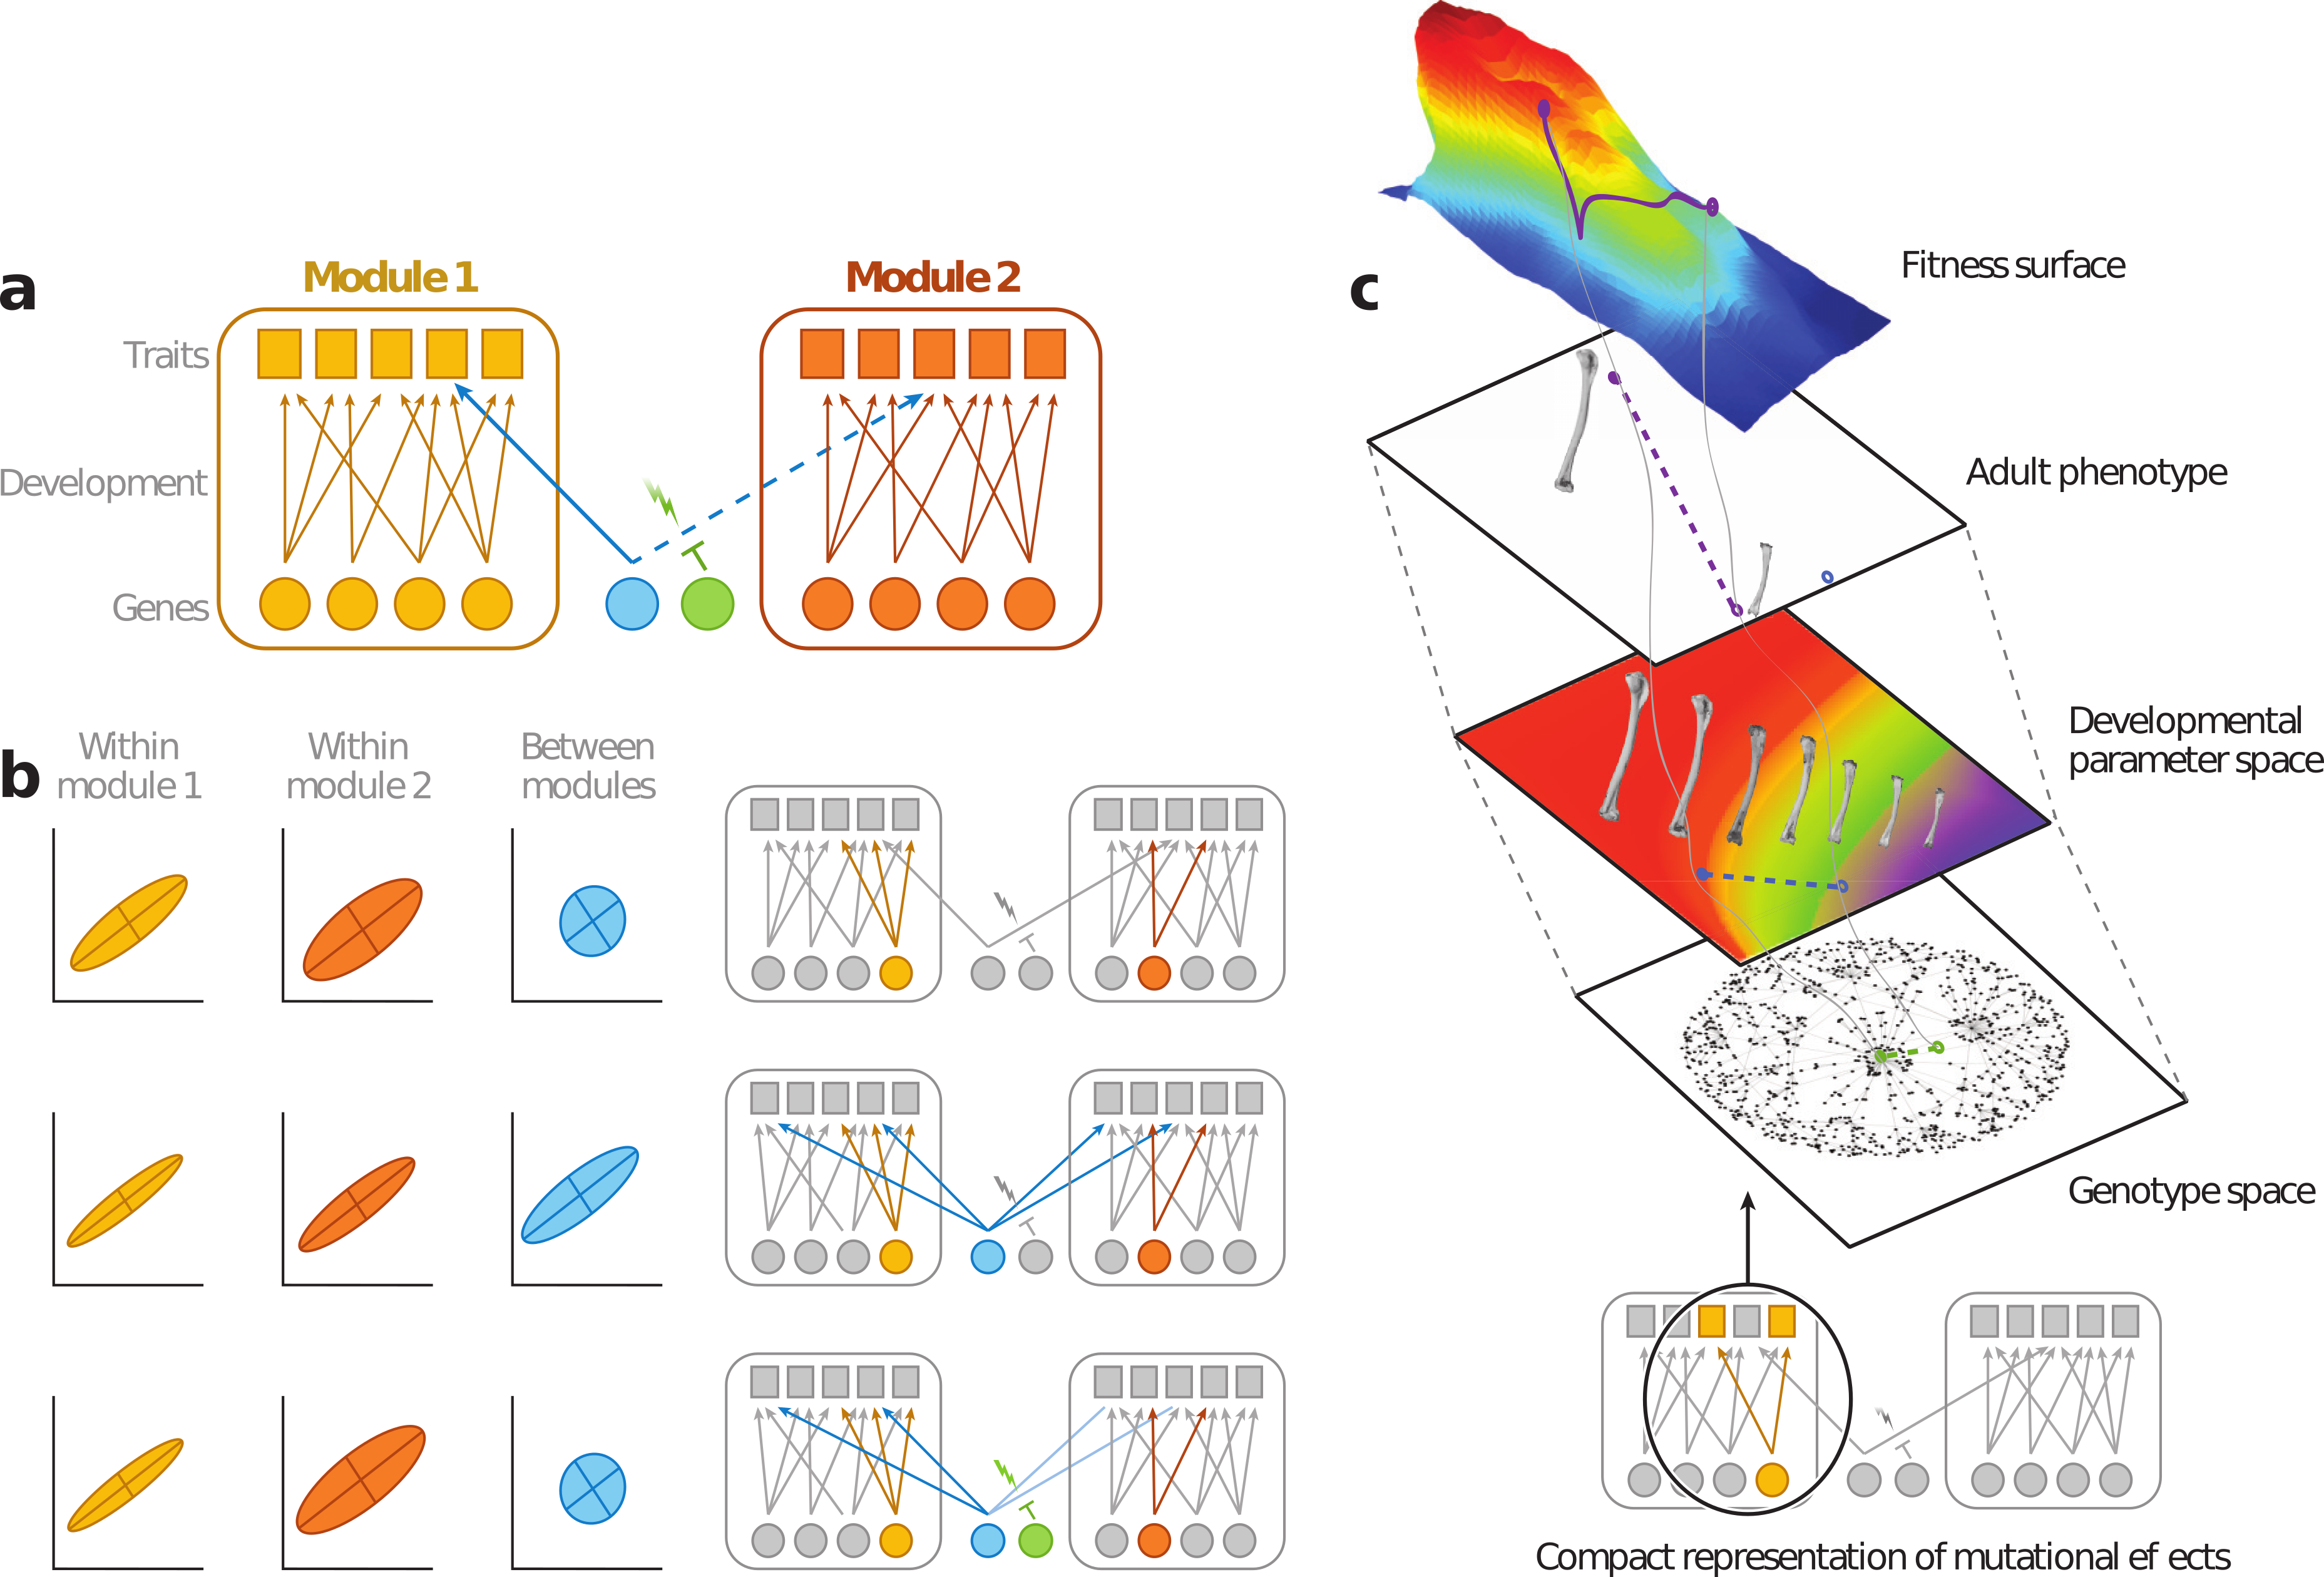
\includegraphics[width=\linewidth]{chapter_annual_review/media/figure1.png}
\caption[Genetic variation in modularity]{(\emph{a}) Typical representation
of modularity in the genotype-\/-phenotype map. Yellow and orange
circles represent modular genetic factors, and blue circles represent
global ones. The green circle represents a genetic locus capable of
preventing the global factor from affecting module 2 (rQTL). Squares
represent phenotypic traits, and arrows represent the relationship
between genotype and phenotype (polygeny and pleiotropy). (\emph{b})
Trait correlation as a function of the underlying genetic variation. In
case 1 (first row), genetic variation is only present for local factors.
Consequently, modular patterns of covariation emerge in the phenotype.
In case 2 (second row), genetic variation in both global and local
genetic factors is present. Consequently, covariation patterns are less
modular. Finally, in the third case, modular covariation patterns emerge
again as a consequence of the rQTL preventing the global genetic factor
from affecting module 2. (\emph{c}) The nature of gene effects across
the different levels of the biological hierarchy. In this panel, we
present a case in which a certain mutation, represented at the level of
the genotype, causes changes in the developmental parameter space (e.g.,
rate of cell division), which in turn leads to changes in the selected
phenotype and movement along a fitness surface. Abbreviation:
relationship quantitative trait loci (rQTL).}
\label{aree:fig1}
\end{figure}

A clearer picture of whether GP maps are modular and whether they
promote the evolvability of organisms came with the collection of large
empirical data sets in mice, yeast, and nematodes (see
\textcite{Wang2010-da}). These large data
sets allowed for a systematic investigation of the pleiotropic effects
of genes on the phenotype across a variety of approaches, including
quantitative trait loci (QTL) mapping and gene knockout studies. The
picture emerging from these large data sets is that most mutational
effects are modular, with different sets of genes affecting different
sets of functionally and developmentally related traits
\parencite{Wang2010-da}. In other words,
the variational modularity observed in the phenotype can be explained by
modularity in the GP map (sensu \textcite{Wagner1996-ui}). A minority of mutations affect large groups of
traits as they are associated with global genetic factors
(Fig. \ref{aree:fig1}). More importantly, in
these same studies, modular pleiotropy was shown to maximize the rate of
adaptation and promote the evolution of complexity, owing to the scaling
of mutational effects with the degree of pleiotropy \parencite{Wang2010-da}.\enlargethispage{\baselineskip}

\section{Evolution of modularity}

\subsection{Genetic Variation in Pleiotropy}

Modularity can evolve through changes in the pleiotropic effects of
alleles on traits themselves. Genetic variation in pleiotropy has long
been recognized as playing an important role in evolutionary processes.
\textcite{Mayr1963-eq} noted the importance of
epistatic interactions in ameliorating the deleterious pleiotropic
effects of alleles on fitness and enhancing their positive fitness
effects. Variation in allelic effects at a target locus is produced by
differential epistasis, a phenomenon in which epistatic interactions
between the target and modifier loci on multiple traits differ in their
effects from one trait to the next \parencite{Cheverud1996-fm, Pavlicev2008-jy, Pavlicev2011-yg}
. Several examples of differential epistasis have been recognized during the last 30 years.
The abnormal abdomen (\emph{aa}) locus in \emph{Drosophila mercatorum}
is a classic example of this phenomenon. In laboratory experiments, the
\emph{aa} locus was found to have a wide variety of pleiotropic effects
on morphological and life history traits \parencite{Templeton1985-ii}
, but these
effects were not manifested in wild populations due to modifier loci.
Differential epistasis has also been described in several other systems,
including coronary artery disease \parencite{Maxwell2013-fe}
 and viral
reproductive success \parencite{Pepin2006-se}.

Although the importance of epistasis has long been appreciated in
evolution, only recently has the major part that epistatic pleiotropy
plays in shaping covariation become apparent.
\textcite{Wolf2005-nr} used QTL mapping
in experimental crosses of inbred Large (LG/J) and Small (SM/J) mice
strains to investigate the genetic architecture in several late and
early skull traits. Covariation between traits was strongly affected by
epistatic variation in pleiotropy, and the genetic architecture
determining the pattern of association between traits can be attributed
to a complex pattern of genetic interactions. In these mice, most
epistatic effects on pleiotropy reduced covariation and led to a more
modular genetic organization. Pavlicev et al. (2008) investigated the allometric relation between body weight and long bone length in mice, and the authors identified several
relationship QTLs (rQTLs), which are QTLs that do not necessarily affect
the mean value of traits but affect the relationships between traits
\parencite{Wagner2007-cx}. This widespread
evidence of genetic variation in the covariation between traits due to
epistatic interactions provides ample scope for natural selection to
change associations between traits and, hence, modularity patterns.

\subsection{Modeling Changes in Covariation}

The availability of variation in the associations between traits led
\textcite{Pavlicev2011-wz} to develop a
deterministic model for the evolution of pleiotropic gene effects under
directional selection. In this model, there is genetic variation in the
strength of the correlation between two continuous traits in the form of
a polymorphic rQTL that has no effect on the trait mean. Traits that are
selected in the same direction tend to become more strongly correlated,
even if selection is fluctuating. Conversely, if the two traits are
under corridor selection, in which one of the traits is selected to
either increase or decrease and the other is kept constant, the rQTL
allele representing low correlation is positively selected and the
traits become independent. The main conclusion of their model is that
the nature of pleiotropic allelic effects is expected to evolve to match
adaptive patterns of selection.

Using the existence of variation in pleiotropic relations,
\textcite{Melo2015-bk} developed an
explicit individual-based stochastic model for the evolution of
continuous traits in finite populations, in which pleiotropic
associations between genetic loci and phenotypic traits are free to
change under mutation. This model has the advantage of being able to
include a number of complications, such as a large number of traits,
drift, different patterns of selection, recombination, and mutation. The
possibility of simulating several traits is especially interesting
because it permits the investigation of complex modular patterns. The
authors evaluated the evolution of modularity under a series of
evolutionary scenarios and reached a number of conclusions. Drift and
stabilizing selection were not capable of creating lasting modular
patterns of covariation, whereas divergent directional selection (during
which one group of traits is selected in one direction and another group
is selected in the opposite direction) created modularity---traits
selected in the same direction became more strongly correlated and
formed clear variational modules. Under corridor selection, the group of
traits under directional selection becomes more correlated, whereas the
group of traits under stabilizing selection maintains intermediate
levels of correlation, and the correlations between these two groups
become very low. These findings suggests corridor selection is a
powerful mechanism for creating complex modular patterns.

Epistasis has also been implicated in the evolution of the mutation
matrix for continuous traits. In \textcite{Jones2014-wj} the authors developed a model for the evolution of two
continuous traits under genetic control of several pleiotropic loci. The
model also included a stable pattern of epistatic interaction between
the loci affecting the quantitative traits. The traits were subjected to
correlated and independent stabilizing selection. Under uncorrelated
selection the traits presented correlations near zero, and the mutation
matrix also had zero correlations between traits. Under correlated
stabilizing selection, however, the traits' genetic correlations changed
and mirrored the pattern of stabilizing selection. The mutation matrix
also aligned with the selection surface and led to a situation in which
the effects of new mutations are biased by previous selective history.

These different models allow us to draw general conclusions regarding
the expected evolution of covariation between quantitative traits,
regardless of the specific model used. First, variation in pleiotropic
relations is essential to the evolution of modularity, and this
variation can be attained through epistatic interactions. Second, under
directional selection, traits that are jointly selected in the same
direction tend to become more strongly correlated. Third, because
selection can change the pleiotropic and developmental relations between
traits, future evolutionary changes can be biased by previous selective
history.

\subsection{Empirical Evidence for Changes in Covariation}

Several instances in which evolution, and presumably selection, has
broken down patterns of association among traits to produce major
adaptive shifts have been reported.
\textcite{Hallgrimsson2012-xw} classified these changes in patterns of modularity as a form of
evolutionary novelty, as there is ``a breakdown of ancestral
developmental constraints such that variation is generated in a new
direction or dimension.'' Indeed, this type of novel variation has been
documented in several systems. \textcite{Young2005-nk} found a common pattern of strong covariation
between the forelimb and hindlimb elements in quadrupedal mammals that
constrains the independent evolution of the limbs. However, two mammals
with highly derived limb morphologies, the brachiating gibbons and the
flying bats, show a reduction in the cross-limb correlation that
accompanies their extreme limb individuation.

Examples of artificial selection overcoming the initial pattern of
genetic associations have also been found. \textcite{Beldade2002-vf}
 used the
eyespots in butterfly wings as a target of selection. Initially, the
anterior and posterior eyespots were correlated, and selection for
coordinated change of both eyespots produced a rapid and linear
response; whereas selection in the uncoupling direction, for increase in
one eyespot and decrease of the other, lead to a response that was much
less linear and more irregular. This study illustrates that there are
preferential directions for evolution produced by the pattern of
modularity, and that evolution is faster in these directions, but these
are not absolute restrictions. Similar results were obtained for
artificial selection experiments aimed at reducing between-sex genetic
correlations for flower size in \emph{Silene latifolia}
\parencite{Delph2011-bc}. Recently,
artificial selection experiments using \emph{Drosophila melanogaster}
revealed yet another important role for selection in influencing
patterns of association among traits. By selecting on allometric
relationships in drosophilid wing shape,
\textcite{Bolstad2015-qr} produced
laboratory lineages presenting larger differences in allometric slopes
than the ones observed across a large clade of drosophilids. This
evolutionary response to selection in the allometric slopes was,
however, quickly lost after selection pressures were suspended. This
finding indicates that internal selection might be responsible for
maintaining conserved allometric slopes on a macroevolutionary
timescale.

These results illustrate the complex interactions between modularity and
selection. Evolutionary restrictions imposed by genetic associations are
rarely absolute, and selection that privileges uncoupling of associated
traits can lead to a reorganization of variational patterns. At the same
time, covariation patterns can also be largely maintained due to either
internal selective pressures (as in the allometric relations in
drosophila) or differences in the availability of rQTL variation to
change pleiotropy.

\section{Development as the Link Between Genes and Phenotype}

Understanding the mechanics and regulation of development is becoming
increasingly essential to elucidating the relationship between
modularity and trait evolution (e.g., \textcite{Salazar-Ciudad2010-wc}).
Development occurs not only through the molecular interaction among many
gene products in a particular environmental context but also through the
mechanical interactions between the developing cells and tissues, all of
which can create significant non-linearities in the GP map \parencite{Alberch1991-sf, Polly2008-bb, Watson2014-pi}. 
In this section, we review recent literature that explicitly addresses the connection
between quantitative approaches to modularity and the underlying
developmental genetics. We are particularly interested in studies that
explicitly incorporate the mechanics of development into an evolutionary
framework or that identify genes that contribute to change in
canalization. We also highlight the emergence of the new field of system
genetics.

\subsection{Causes of a Phenotype Versus Causes of Phenotypic Variation}

In a developmental context, it is particularly important to distinguish
between the causes of a phenotype and causes of phenotypic variation. A
developmental process might be essential for a trait to emerge (cause of
a phenotype), but as long as this process is conserved across
individuals, it will not be a cause of phenotypic variation in a
population. Empirical evidence overwhelmingly suggests that causes of a
phenotype are modular in nature. The whole concept of character relies
on it. According to \textcite{Wagner2007-zs},
character identity is specified by gene regulatory units that control
the developmental program. These regulatory units, termed character
identity networks, imply that we can truly recognize something as a
distinct character only if it shows some degree of modularity at the
developmental genetic level.

Modularity in the causes of variation of a phenotype is another matter
altogether. The notion that causes of phenotypic variation might also be
modular stems from the concept of morphological integration, as seen
above (section \emph{Genetics of modularity}), and from the imitatory
epigenotype hypothesis \parencite{Riedl1978-ub},
which predicts that the pattern of developmental constraints imitates
the pattern of functional constraints, thereby leading to covariation
among functionally related traits within populations. Empirical evidence
suggests that there can be a correspondence between variational and
developmental modularity, but this correspondence is by no means
guaranteed, as seen in previous sections.

\subsection{Incorporating Development into Evolutionary Studies}

Although variational modularity is often assumed to be a consequence of
variation in the underlying developmental mechanisms, explicitly
modeling developmental systems or even inferring developmental processes
from variational modules are not simple tasks \parencite{Hallgrimsson2009-kq, Pavlicev2015-up}.
Interactions among tissues, as well as local and global genetic factors
acting at different time points, are all superimposed during development
and contribute to the final phenotype \parencite{Hallgrimsson2009-kq, Mitteroecker2007-xq}.
Similarly, a single modular pattern can emerge through multiple
independent developmental pathways \parencite{Mitteroecker2009-jb}
 and make the
prediction across levels of the hierarchy difficult. To our knowledge,
the most successful empirical case of incorporating developmental
parameters in evolutionary models is \textcite{Salazar-Ciudad2002-yf, Salazar-Ciudad2010-wc}
 model of tooth development.
Tooth development is a relatively well understood process, as several of
the genetic interactions and cellular processes that lead to tooth
formation are known. Consequently,
\textcite{Salazar-Ciudad2010-wc}
created mathematical models describing tooth morphology as a consequence
of perturbations in the underlying genetic and developmental parameters,
such as the rate of cell proliferation or cell adhesion. This model was
successful at producing accurate predictions of tooth morphology for
several mammalian groups
\parencite{Salazar-Ciudad2010-wc}.
Other successful cases of the use of developmental mechanisms to explain
phenotypic variation comes from \emph{Drosophila} wing venation patterns
\parencite{Matamoro-Vidal2015-vd} and
butterfly wing eyespots \parencite{Beldade2002-vf}, both of which involve changes in several key
developmental processes, such as the distribution of morphogens in the
wing disc or the establishment of planar cell polarity.

A theoretical approach that has also undertaken a more explicit
incorporation of developmental information into the evolution of the GP
map was developed by \textcite{Watson2014-pi}. In their model, multivariate traits are produced by a GP map
with multiple independent developmental steps connecting the phenotype
to the genotype. This conceptualization produces a nonlinear ontogeny
and allows the model to capture interesting behaviors of these GP maps,
such as the ability to recall multiple phenotypes that were selected in
the past or the ability to produce new combinations of features from
modular developmental processes. Traits in this model tend to become
more associated throughout development when they are selected in the
same direction and become independent when they are selected in
different directions, thereby reinforcing the role of directional
selection in shaping modularity.

\enlargethispage{\baselineskip}
In conclusion, although approaches relating variational modularity to
the mechanics of development are relatively rare, these different
empirical studies and theoretical models clearly show that incorporating
the more complex developmental interactions into studies of
morphological variation and evolution greatly increases our ability to
understand and even predict the evolutionary dynamics of complex
systems. The main challenge going forward will be to create models
capable of describing more complex structures, such as the skull;
allowing specific connections between DNA sequences, developmental
networks, and variational modularity; and incorporating the possibility
of changes in the topology of genetic and developmental networks.

\subsection{System Genetics---A Systematic Approach}

A promising way to integrate modularity with the underlying
developmental genetics in a systematic way is currently gaining traction
with the system genetics approach \parencite{Ayroles2009-ld, Mackay2009-fo}. 
The idea behind
system genetics is simple. It interrogates the relationship between
genome and phenome under different contexts (e.g., environments or
conditions). Consequently, it attempts to hit at the core of the context
dependency of gene effects, which not only is fundamental for the
evolution of modularity \parencite{Pavlicev2015-up}, as seen in previous sections, but also emphasizes its
developmental basis by potentially uncovering important modular
signaling cascades.

System genetic approaches have been applied to several different model
organisms \parencite{Ihmels2002-fg, Juenger2005-uc, Wang2010-da}. In
\emph{Drosophila} \textcite{Ayroles2009-ld}, it led to the identification of several transcriptional modules
that are not only connected to genomic variation but also underlie
variation in ecologically relevant traits, such as fecundity and
metabolism. Those transcriptional modules are strongly influenced by
environmental, developmental, and genetic background effects, thereby
highlighting the fact that context-dependent effects are the norm and
therefore are responsible for most phenotypic variation. System genetic
approaches have also recently been used to map changes in the amount of
variation for a given phenotype \parencite{Ayroles2015-ab}. Genetic variation in phenotypic variance represents
genetic variation in developmental canalization, a topic that is
especially relevant to studies of threshold characters or threshold
selection \parencite{Ayroles2015-ab}. Among
the challenges faced by system genetics, two should be highlighted. Due
to its ambitious nature of scoring multivariate traits and entire
transcriptomes/genomes, system genetics studies are inherently expensive
studies. Also, multivariate statistics are often dependent on large
samples and are often estimated with considerable error, an aspect that
needs to be taken into account.

\section{Modularity and the Adaptive Landscape}

How is modularity and integration relevant for phenotypic evolution?
Having discussed and characterized modularity and the possibility of its
evolution, we now address its evolutionary consequences. There are
short-term and potentially long-term consequences of modularity for
evolutionary change. We start by introducing the quantitative theory
dealing with the short-term consequences and identifying under which
circumstances this theory can be extended to macroevolutionary time.
Because modularity in patterns of genetic associations between
continuous traits is captured by the additive genetic
variance/covariance matrix, the G-matrix \parencite{Lande1979-by}, this section focuses on
the relationship between the G-matrix and the adaptive landscape, which
relates possible phenotypes in the morphospace with fitness
(\emph{sensu} \textcite{Simpson1944-pf, Arnold2001-lz}).

\subsection{Why So Much Interest in the G-Matrix?}

\enlargethispage{\baselineskip}
Evolution, regardless of which evolutionary process is involved, depends
on genetic variation. The G-matrix summarizes the amount and pattern of
additive genetic variation and covariation among traits and is,
therefore, essential to our understanding of the connection between
genetics and evolution \parencite{Lande1979-by}.
Genetic covariation among traits is particularly important because of
its potential to affect the course of phenotypic evolution
(Fig. \ref{aree:fig2}). Unlike the univariate
view of evolution, in which a single trait's value can be optimized
without constraint from selection on other traits, genetic covariation
among traits causes correlated responses to selection. In this situation
traits will change and evolve together, often in a direction that is
different from the one favored by selection
(Fig.~\ref{aree:fig2})
\parencite{Lande1979-by, Grant1995-er}. Thus, the pattern and
magnitude of the G-matrix elements can deflect the path of evolution
from its optimal trajectory. Whether or not this short-term effect on
the evolutionary responses has enduring consequences depends on the
degree of stability of the G-matrix and on its relationship with the
adaptive landscape [\textcite{Steppan2002-be}; see also section \emph{Evolutionary change in rugged
landscapes}].

Long-term stability of the G-matrix is one of the most fundamental
assumptions of the research program described here, and questions
related to the long-term stability and estimation of G-matrices are
still open \parencite{Houle2015-jb, Jones2012-aq}. Many feel
uncomfortable with this assumption of stability \parencite{Bjorklund2013-io}. This
discomfort stems in part from empirical evidence that suggests that no
two populations have identical G-matrices and that G-matrices can
fluctuate over short time periods \parencite{Bjorklund2013-io, Eroukhmanoff2011-ph}.
Biological populations are finite and almost surely differ in their gene
frequencies, especially considering the potentially large number of
genes affecting complex traits and the correlations between them \parencite{Phillips2001-xb, Whitlock2002-yb}. 
We suggest that in many instances the assumption that population covariance
matrices are identical be rejected out of hand. But the mere presence of
a statistically significant difference is not the critical issue.
Instead, the more interesting and relevant questions are: How similar
are two covariance patterns with respect to their predicted evolutionary
responses? Do some quantitative traits have more stable G-matrices than
others? Fortunately, these are questions that can be examined
empirically \parencite{Calsbeek2009-fl, Cheverud2007-yp} and
are a critical first step for the use of the G-matrix in multivariate
evolution and systematics.

\begin{figure}
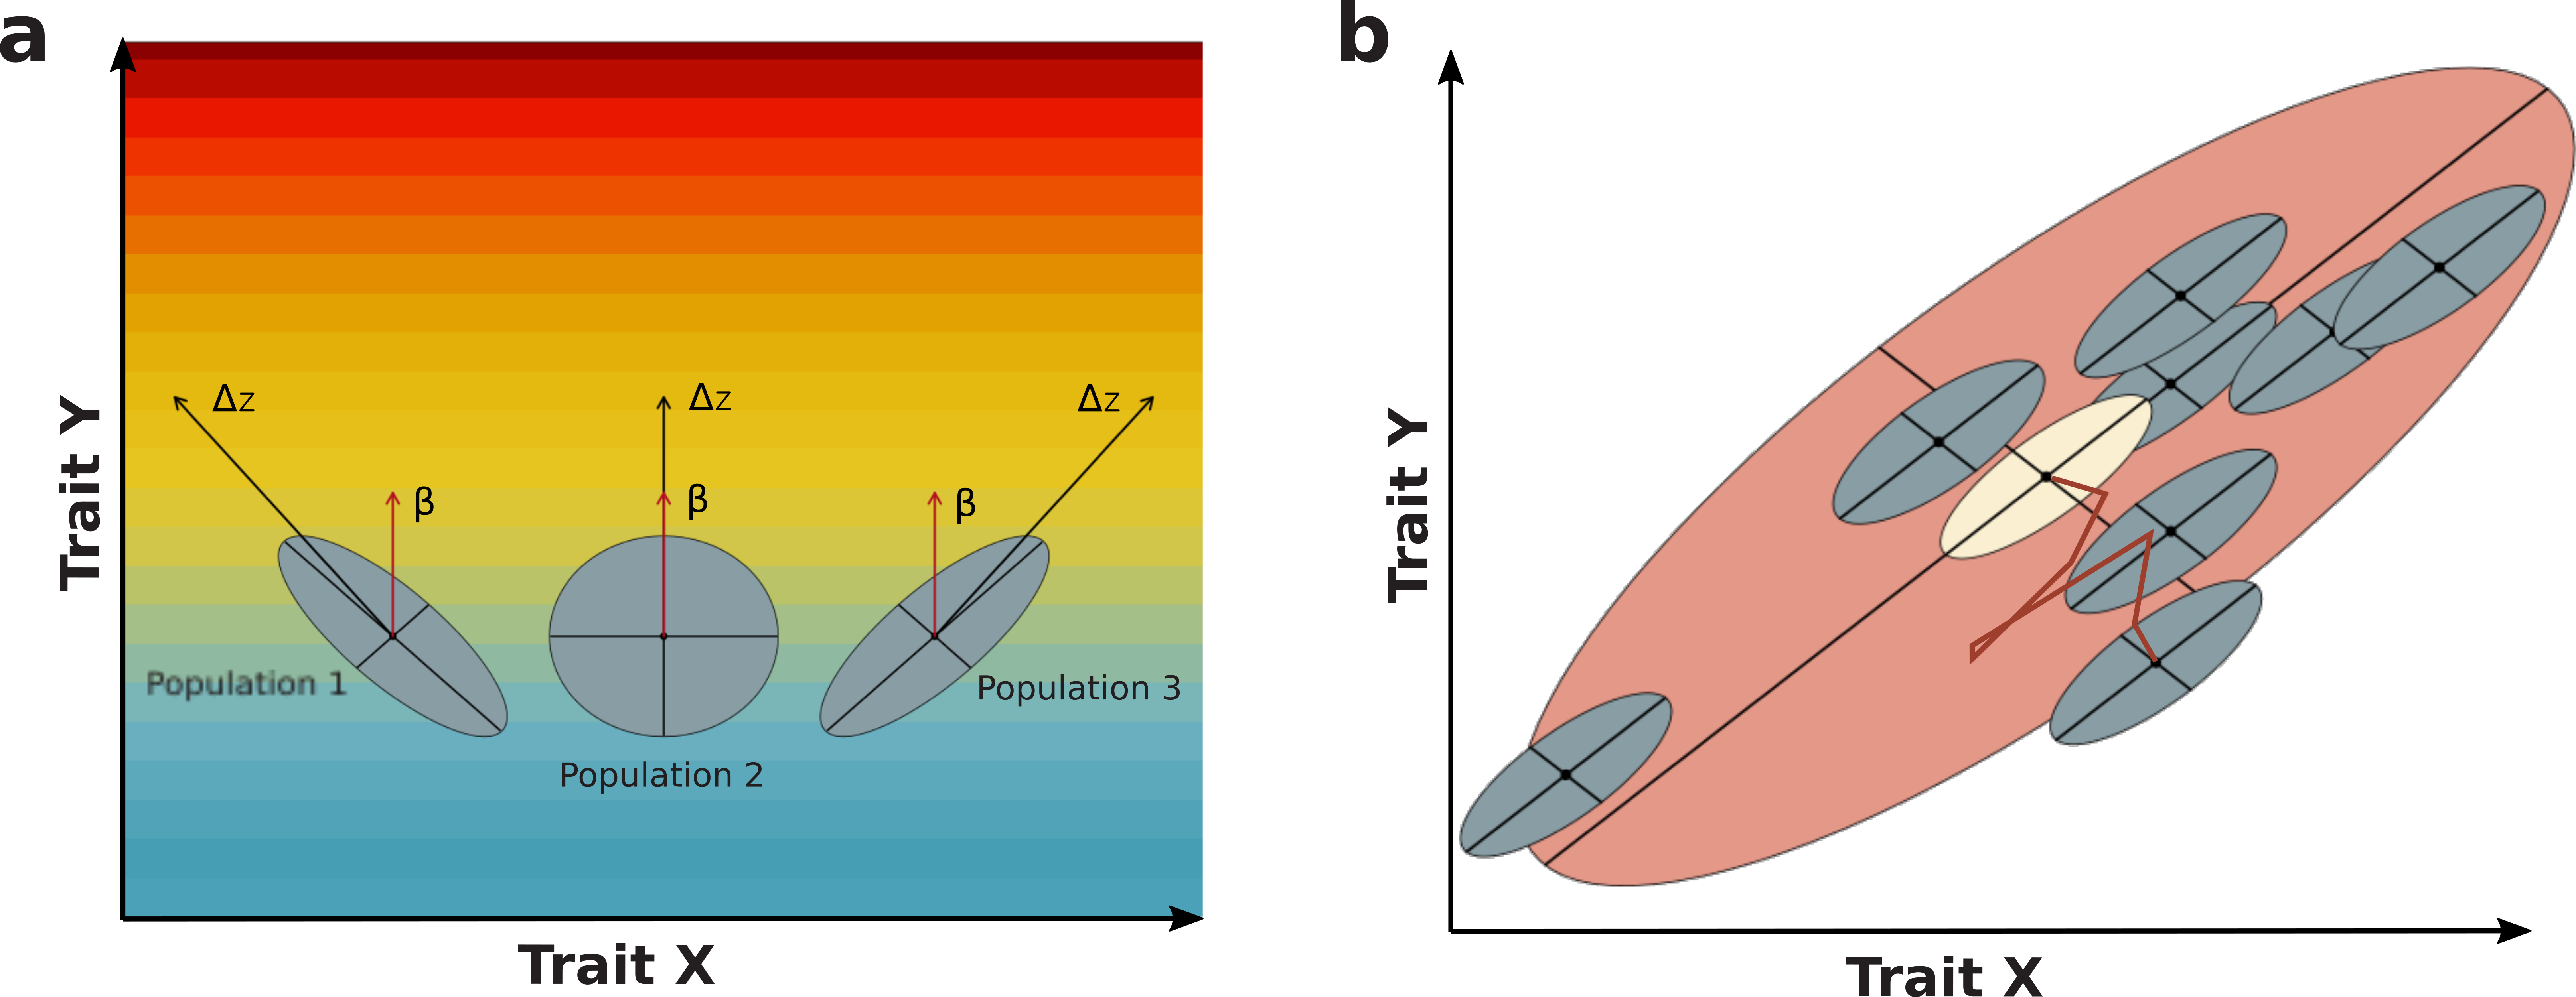
\includegraphics[width=\linewidth]{chapter_annual_review/media/figure2.png}
\caption[Selection, drift and covariation]{To illustrate the interaction of
modularity (captured in the G-matrix) and evolutionary processes
(selection and drift), we display two panels illustrating population
averages, G-matrices, adaptive peak(s), and selection gradients ($\beta$).
G-matrices are represented by ellipses of different colors and with the
axes of major genetic variation embedded. The major axis corresponds to
the line of least resistance \parencite{Schluter1996-gw}, 
that is, the direction which holds most of the genetic
variation in the trait space. Selection gradients are represented by
straight arrows and measure the relationship between fitness and
individual traits while holding the other traits constant. Responses to
selection ($\Delta z$) are also shown as arrows and indicate changes in the
trait averages across time. The multivariate response to selection
equation ($\Delta z = G\beta$) captures the relationship between the response to
selection ($\Delta z$), inheritance (G-matrix), and selection ($\beta$). The direction
of increase in average fitness is indicated by the plus sign (+) and
decrease in fitness is indicated by the minus sign (-). The left panel
shows 3 populations (\emph{green}, \emph{yellow}, and \emph{red}) under
the same adaptive landscape, in which an increase in trait Y is favored
and trait X does not affect fitness. Notice that the response of each
population to the same selection gradient differs (\emph{dark green},
\emph{orange,} and \emph{dark} \emph{red arrows}). Population Green
increases Y but decreases X values, population Red increases Y and X
values, and population Yellow only increases Y, although with a smaller
displacement of Y than the other two populations. These different
responses under the same selection gradient are due to differences in
the G-matrices. Populations Green and Red have their responses deflected
from the optimal path, due to the covariation between Y and X (negative
in Green, and positive in Red). Thus, traits that are not under direct
selection will contribute to the response owing to their shared
inheritance. If traits are independent (population Yellow), each can be
optimized separately. But note that the displacement in the Y average is
smaller than in the other populations, because the genetic variation
available in that direction is smaller. The right panel shows the
consequence of a flat adaptive landscape (random genetic drift) on the
averages of descendent populations (\emph{red ellipses}) of an ancestral
population (\emph{yellow ellipse}). The arrows in this case point to
each population's trajectory. At the end of the drift process, 95\% of
all evolution (divergence among means) is captured by the larger ellipse
(\emph{light pink}). Notice that substantially more divergence appears
along the axis holding most of the within-population genetic variation.}
\label{aree:fig2}
\end{figure}

So, what do empirical studies tell us about the relative stability of
the G-matrix over macroevolutionary timescales? Empirical evidence
varies greatly depending on the study system in question. One of the
most thoroughly explored cases is the mammalian skull, from which
empirical evidence strongly suggests that G-matrices are stable across
mammalian taxa \parencite{Garcia2014-oj, Marroig2001-ne, Porto2009-pi}. By stable we do
not mean that heritable variation patterns are identical across species,
but that they will deflect the phenotypic response to selection in a
similar way.

Although it is possible that extant species variation patterns are
fairly similar, it is also possible that stochastic fluctuations in the
G-matrix over generations are large enough to render the inferences we
might make from extant patterns useless. These fluctuations are possible
for many reasons, like segregating alleles with large effects or linkage
disequilibrium caused by periods of strong fluctuating selection \parencite{Bulmer1971-aa, Turelli1988-io}. 
Although this is certainly a theoretical possibility, the critical question is whether or
not changes in G-matrix structure are of sufficient magnitude to affect
evolutionary inferences \parencite{Arnold2008-pc}. Fortunately, simulations quantifying these problems suggest
that their effect may often be small \parencite{Jones2012-aq, Jones2004-be}.

\subsection{The Missing Link: Adaptive Landscapes and the G-Matrix}

We have discussed genetic associations, the genetic and developmental
origins of modularity, and their influence in evolutionary response. One
missing, and arguably the most important link, is the relation between
covariation and the adaptive landscape. By examining the relationship
between modularity and adaptive landscapes, we can put micro- and
macroevolution into a common unifying theory \parencite{Arnold2001-lz, Arnold2014-gd}. 
This theory not
only explains the relationship between development, function, and
inheritance in shaping modularity patterns but also allows us to explore
the evolution of multivariate phenotypes in deep-time and suggest future
research directions.

Although many studies have been conducted at a local scale
(within-population), we have precious little information about how
adaptive landscapes vary between species \parencite{Pfaender2016-eb}. One of the
most important developments in the past 30 years of evolutionary theory
were the multivariate regression methods for inferring individual
selection surfaces from multivariate data \parencite{Lande1983-ez}. 
Although not
without critics \parencite{Shaw2010-wg},
these methods have allowed researchers to directly investigate adaptive
landscapes and to empirically measure selection on multivariate trait
sets. In this approach, the adaptive landscape is described by two main
terms: a linear term related to directional selection and a quadratic
term related to stabilizing/disruptive selection \parencite{Lande1983-ez}. 
The quadratic
component affects the variances and covariances among traits and, along
with directional selection, is thought to be the major evolutionary
process shaping modularity \parencite{Melo2015-bk}. The selection gradient (linear term) is the direction
of maximum increase in fitness and is the vector of partial regression
coefficients of fitness on traits. This framework can also be used to
study directional selection retrospectively: By measuring extant species
means and covariance matrices we can estimate ancestral states and, by
solving the Lande equation, the selection gradient that would have
resulted in the observed diversification can be estimated
(\textcite{Lande1979-by}, equation 9)
(Fig.~\ref{aree:fig2}).

Even though this toolkit for explicitly characterizing selection has now
been available for decades, empirical characterizations of multivariate
selection are still rare, despite their acknowledged importance. Yet the
past 20 years of reconstructing selection gradients from extant
diversity have given us two fundamental insights into the nature of
multivariate evolution. First, estimates of the strength of both
stabilizing and directional selection are usually weaker than we
previously assumed \parencite{Kingsolver2001-yq, Kingsolver2012-yv}. But, more importantly,
the empirical evidence suggests that the direction of evolutionary
divergence and the direction of selection are rarely the same and, often
times, present little resemblance (see the section, Does Alignment with
Lines of Least Resistance Imply Constraint?). An important work
illustrating this notion comes from studies of \emph{Drosophila serrata}
\parencite{Chenoweth2010-dg}. In a study of
sexual selection, the authors note that even though local processes of
sexual selection varied considerably across their nine populations,
evolutionary divergence occurred primarily along a single trait
combination. Variation in sexual selection had little influence on
evolutionary divergence. Instead, genetic covariation among traits
caused the evolutionary response to be significantly deflected from its
optimal path. Studies on \emph{Dalechampia} blossom morphology have also
emphasized that only a portion of evolutionary divergence patterns can
be accounted for by estimates of external selective factors, such as
community composition and availability of resources. Rather, constraints
imposed by covariation patterns seem to be essential for our
understanding of the evolution of blossom traits \parencite{Bolstad2014-oi, Hansen2006-yc}.

We should point out that selection gradients reported in these
retrospective works are net gradients, that is, estimates of the
cumulative sum of all selection gradients acting over the generations of
divergence. If the G-matrix is stable, this net selection should be a
reasonably accurate estimate of the sum of individual gradients \parencite{Jones2004-be}. 
Another issue
with reconstructing selection is that G- and P-matrices are often
estimated with substantial error, frequently resulting in poorly
conditioned or negative semidefinite matrices. Thus, the inversion step
in the reconstruction analysis can lead to very large errors \parencite{Marroig2012-jd}. 
Fortunately,
matrix estimation or regularization methods can vastly improve the
selection gradient estimates, and these methods should be used whenever
selection estimates are made \parencite{Marroig2012-jd, Schafer2005-ld}.

\subsection{Evolutionary Change in Simple Landscapes}

Most of our knowledge of the relationship between modularity and the
adaptive landscape comes from simulation studies. In simulations carried
out on simple landscapes, patterns and magnitudes of association among
traits affect the direction, magnitude, and rate of evolutionary change
under selection (e.g., \textcite{Marroig2010-be}). The effect of the G-matrix on evolutionary change
depends critically on its structure in relation to the adaptive
landscape \parencite{Conner2012-ru, Laughlin2015-od} and can
either augment or slow the evolutionary response relative to a situation
with fully independent traits. If selection is along dimensions
unaligned with modularity/integration patterns, the response is
deflected toward the lines of least resistance \parencite{Schluter1996-gw}. If selection is
aligned with modularity, however, the evolutionary response is greatly
facilitated \parencite{Beldade2002-vf, Bolstad2014-oi}. The closer the
alignment with the major line of least resistance, the quicker and more
direct the evolutionary response. However, simulations are highly
concordant in showing that these effects are restricted to the
microevolutionary scale, and, given sufficient time and a simple
adaptive landscape, the population will eventually reach the selective
peak, unless there is no genetic variation at all in that direction (an
absolute constraint) \parencite{Blows2005-sd}. But theoretical work suggests that even if there is an apparent
lack of genetic variation along some dimension, genetic variation is
frequently hidden in the form of epistasis that can fuel evolutionary
change in subsequent generations \parencite{Hansen2013-vy, Hansen2006-yc}.
Therefore, given the possibility of adaptive changes in the G-matrix
through time and the understanding that constraints imposed by
G-matrices are usually microevolutionary, the emerging picture would be
one in which G-matrices should not have any enduring macroevolutionary
consequences (termed the transient constraints model, from now on). But
what happens when we consider complex adaptive landscapes?

\subsection{Evolutionary Change in Rugged Landscapes}

Although single-peaked adaptive landscapes are convenient for model
building purposes, adaptive landscapes are thought to be very rugged,
that is, they have many adaptive peaks and valleys \parencite{Kauffman1987-ds, Martin2013-ez, Wright1932-ve, Pfaender2016-eb}. When the adaptive
landscape is rugged and genetic associations are stable through time,
macroevolutionary dynamics are shaped by the interaction between the
G-matrix and the adaptive landscape
(Fig.~\ref{aree:fig3}). This interaction implies
that, in rugged and multiple-peaked adaptive landscapes, the G-matrix
can have a major influence in determining which peak will be reached by
a given population, even if in theory the effect of the G-matrix is
microevolutionary \parencite{Steppan2002-be}. This argument was already present in
\textcite[p.~407]{Lande1979-by} but in a somewhat
opaque formulation: ``[However,] the adaptive topography for each
population or species generally has multiple peaks\ldots{}. Genetic
correlations can alter the long-term result of selection by influencing
the direction of evolution at critical periods when a population
approaches a threshold (or saddlepoint) between adaptive zones, as by
random genetic drift or by environmental fluctuations which directly
affect the phenotype or alter the adaptive topography.'' This argument
can be easily understood noting that, in evolutionary terms, the
distance between the population average position and the peak is not a
simple linear (Euclidean) distance between the start position and end
position of the species averages but is a weighted distance, with the
weight being given by the patterns of genetic association. Given the
influence of genetic correlations, the distance of a population from a
peak is measured in units of genetic variation. Thus, the closest peak,
the peak the population eventually reaches, is not necessarily the
highest or even the closest in Euclidean distance but is the closest in
genetic-scaled distance. We refer to this idea as the peak selection
model.

\begin{figure}[ht]
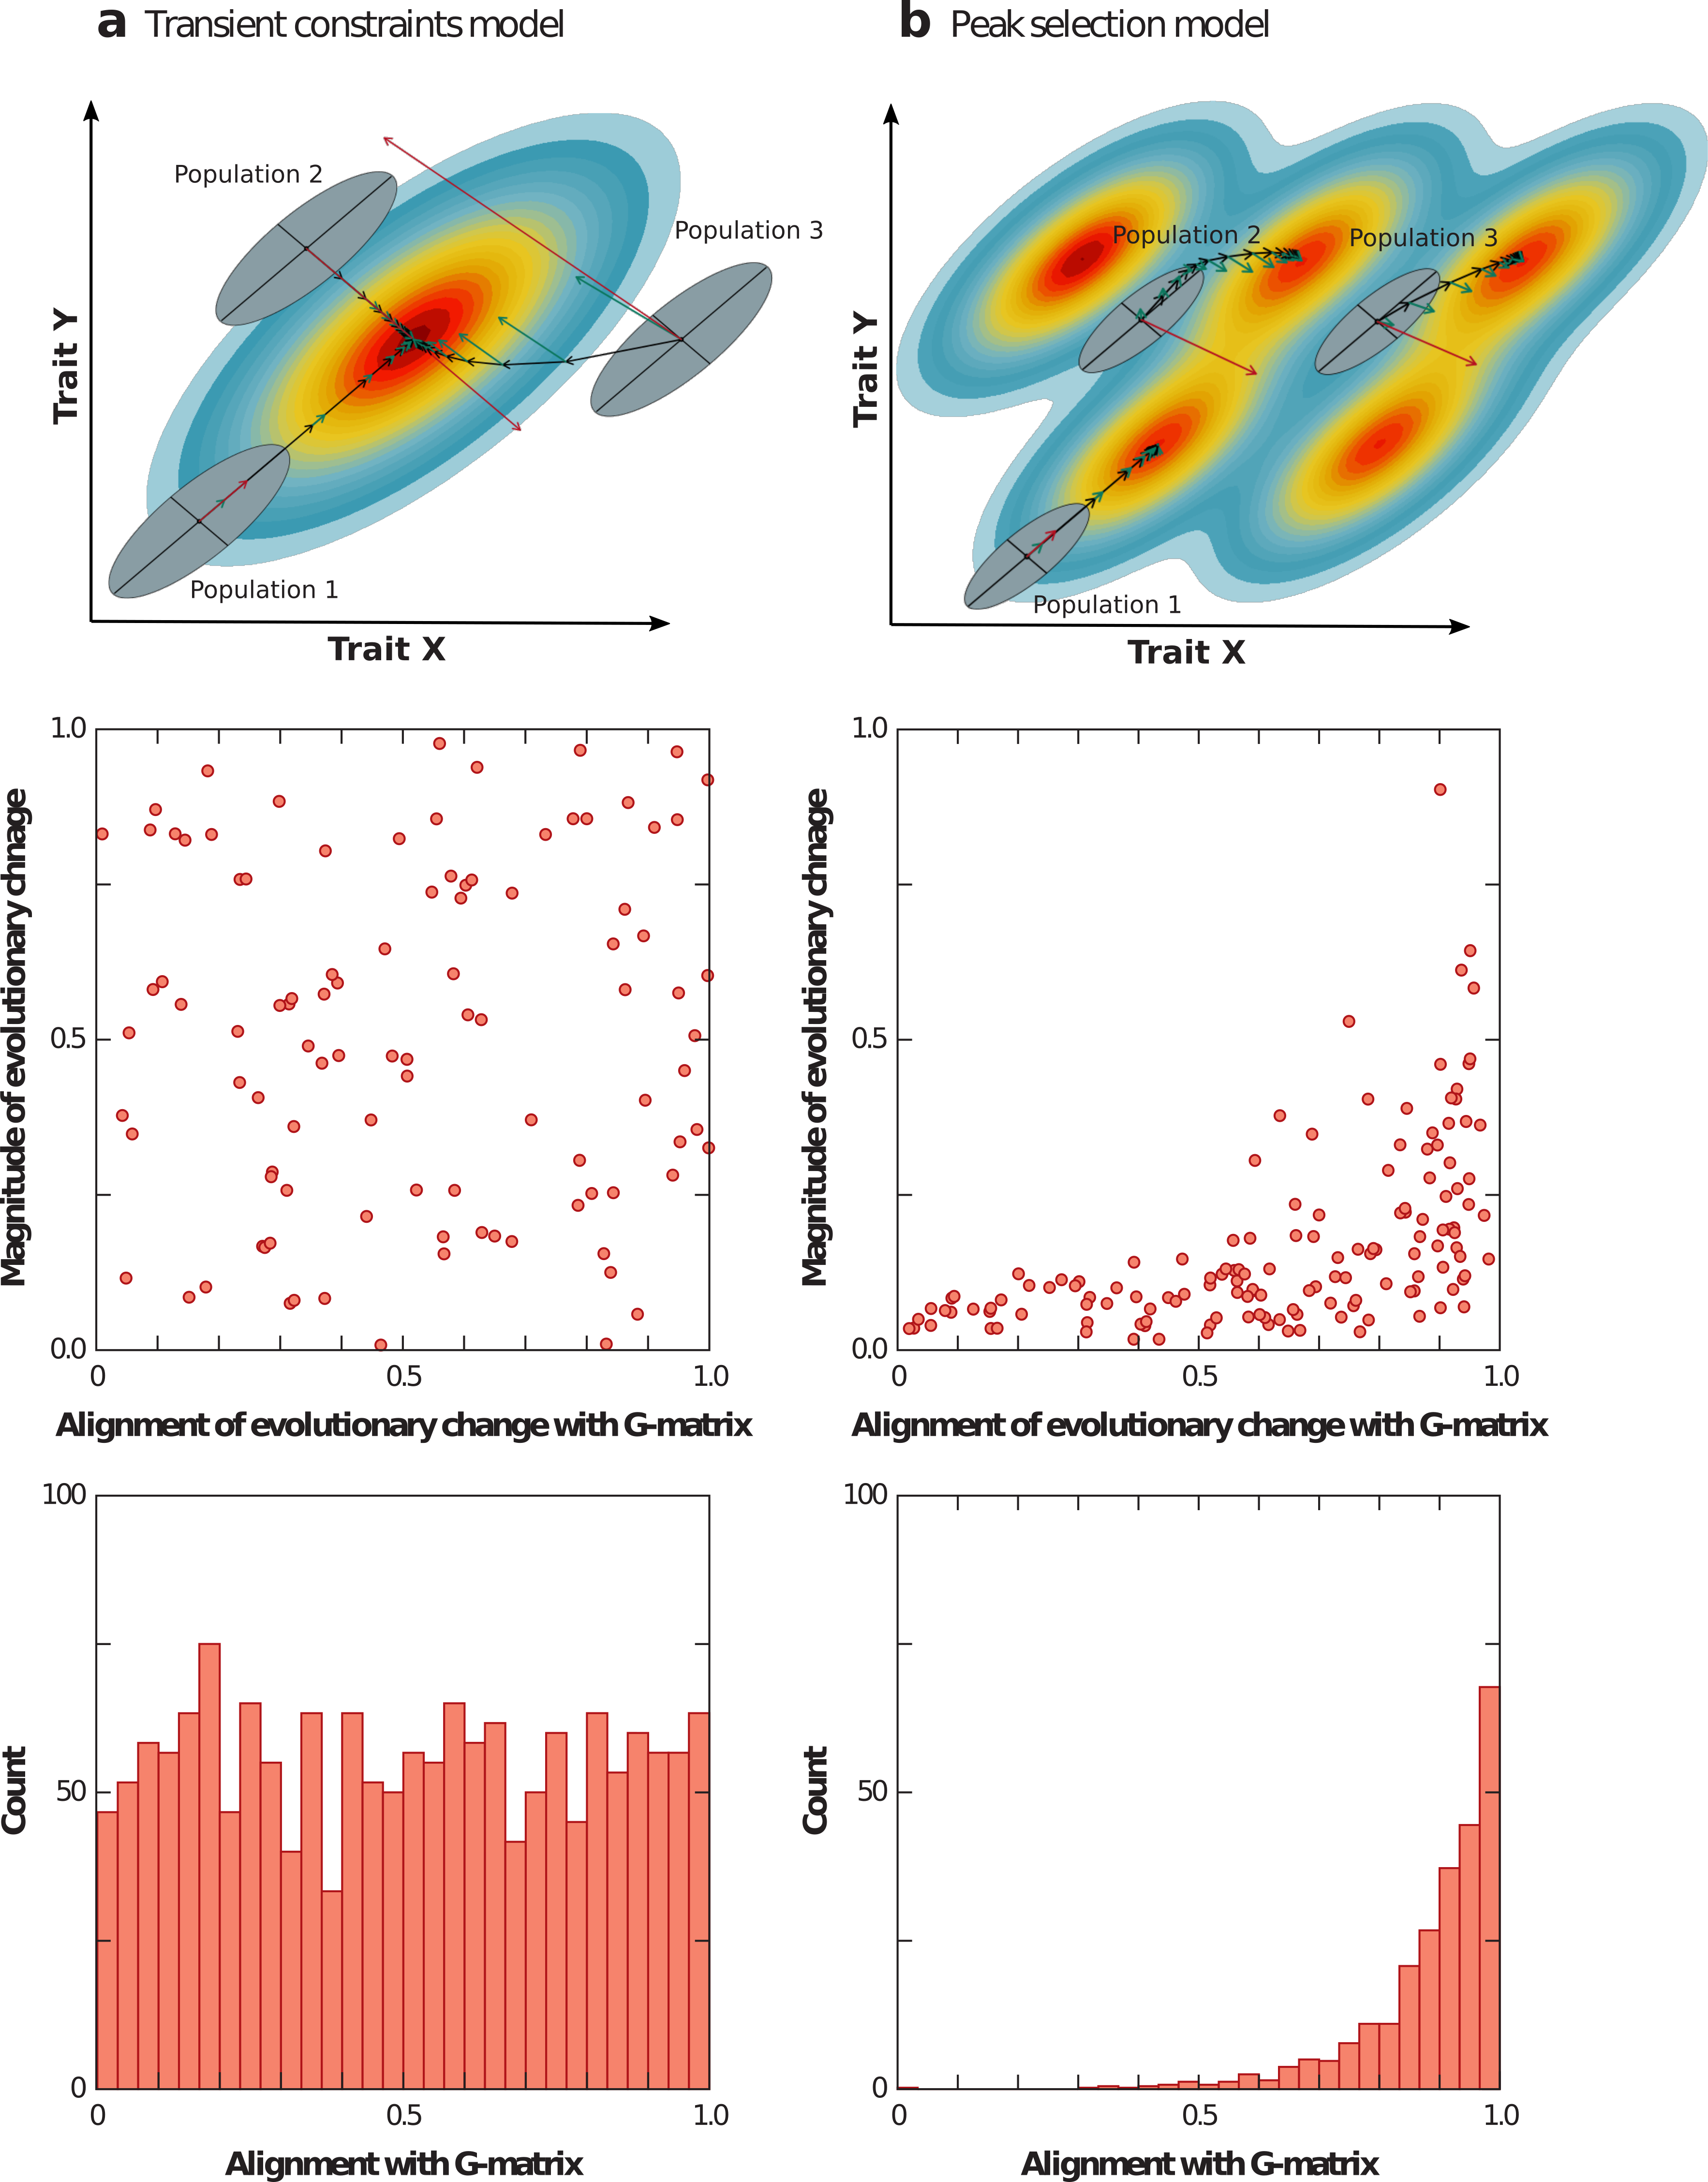
\includegraphics[width=\linewidth]{chapter_annual_review/media/figure3.png}
\caption[Single peak vs. multiple peak selective landscapes]{Left panels (\emph{a}) show the transient constraints model, and right panels (\emph{b}) show the peak selection model. 
Top left panel shows selection gradients ($\beta$) per generation (\emph{green arrows}) and average responses ($\Delta z$) per generation (\emph{black arrows}) of populations sharing similar G-matrix structure but at different starting points of a single-peaked adaptive landscape. 
Red arrows represent the net selection gradient (the sum of all selection gradients). 
Thus, the alignment between the direction of selection and the orientation of the G-matrix differs for each population. 
Responses to selection will thus vary between populations, in terms of direction and magnitude. 
Some populations will evolve rapidly and directly to the peak (\emph{population 1}), whereas others will evolve slowly (\emph{population 2}) owing to differences in the amount of variation aligned with selection (evolvability sensu \textcite{Hansen2008-kz}) (\emph{Continues}). 
\label{aree:fig3}
}
\end{figure}
\begin{figure}[ht]
  \contcaption{Population 3 will approach the peak in a nonlinear way, and its trajectory will be strongly deflected by the G-matrix in the direction of the line of least resistance. 
The line of least resistance equals the first principal component of a G-matrix and acts as an attractor of short-term evolutionary responses.
We can expand this notion to multivariate systems and think of linear combinations of the first principal components as representing hyperplanes of least resistance. 
This notion is related to modularity, because principal components are related to modules but do not carry a one-to-one relation with each module \parencite{Berner2011-bi}. 
Usually, principal components are contrasts between modules (positive loadings for one module and negative loadings for the other), and linear combinations between these contrasts define directions of independent change for each module. 
Note that the net selection gradients (\emph{red arrows}) are much larger when selection is not aligned with the G-matrix’s main axis. 
The top right panel shows the same three populations but in a rugged adaptive landscape. 
In this scenario, populations won’t always evolve to the closest peak (Euclidean distance) but instead will evolve to those that are closest given the covariation among traits. The central panels illustrate the predictions of each model (transient constraints, \emph{left}; peak selection, \emph{right}). 
Each point represents one species, with Y being the total magnitude of evolution, and X being the alignment of the evolutionary response ($\Delta z$) with the G-matrix. 
In the transient constraints model (\emph{a}), you would not expect any particular relationship between the magnitude of evolutionary change and its direction, because every species would eventually reach the peak. Conversely, under the peak selection model (\emph{b}), species’ evolutionary trajectories may or may not be aligned with the G-matrix, but the magnitude of evolutionary change will be small when not aligned. Bottom panels show the predictions for both models (transient constraints, left; peak selection, right) of the number of species observed in terms of their evolutionary response ($\Delta z$) and their alignment with the G-matrix.}% Continued caption
\end{figure}

What would we expect in terms of empirical patterns under each of these
scenarios? If G-matrices impose only microevolutionary constraints and
population/species eventually reach their single-adaptive peak, we would
expect no particular relationship between the magnitude and direction of
evolutionary change and its alignment with the G-matrix. We would also
not expect any significant alignment of the species response to
selection with the major axis of variation of the G-matrix. Evolution in
this scenario would depend only on the position of the adaptive peak in
relation to the population average. Alternatively, if G-matrices have
enduring consequences at the macroevolutionary level by influencing the
choice of peak, we would expect an association between the magnitude and
direction of evolutionary change and its alignment with the major axis
of the G-matrix (see \textcite{Porto2015-zv}). Furthermore, species diversification should be biased in the
directions of highest variation in the G-matrix. Evolutionary change
would depend not only on the position of the adaptive peaks in regard to
the current position of the population averages but also on the G-matrix
structure, which would affect the probability of reaching the various
peaks (Fig.~\ref{aree:fig3}). A possible
complication of the single peak model is one in which we have only one
peak, but this single adaptive peak is not fixed, instead fluctuating
randomly in the morphospace over time \parencite{Jones2012-aq}. What would be
the expectations under this model? The answer would depend on the
frequency and magnitude of the peak fluctuation over time, and on
whether or not the G-matrix evolves. If peak displacements are small and
rare, the expectations would be more in line with the transient
constraints model. Conversely, if peak fluctuations are common or large
in magnitude, it is possible that populations never quite reach
equilibrium and traverse the morphospace walking on the line of least
resistance, thus approaching the expectations from the rugged peak
model.

\subsection{Does Alignment with Lines of Least Resistance Imply Constraint?}

Comparisons of G-matrix orientation with the observed direction of
evolutionary change, as described in the previous section, can be a
fruitful way to test these ideas. Several studies have compared
morphological diversification with available genetic variation: In
several instances diversification was aligned with the lines of least
resistance, whereas other instances showed diversification in alternate
directions \parencite{Berner2010-dp, Marroig2010-be, Renaud2006-ds, Schluter1996-gw}. 
But this alignment is
not necessarily due to constraints, because selection and constraint can
act in the same direction \parencite{Conner2012-ru, Marroig2010-be}. This would imply either that species
lie near the axis of major evolvability not due to constraint but to a
ridge in the fitness surface \parencite{Conner2012-ru} or that at least 
some of the available peaks happened to be
aligned with that direction and thus the pattern is adaptive \parencite{Arnold2001-lz, Marroig2010-be}. Likewise, macroevolutionary diversification that is not aligned with variation
does not negate the possibility that the G-matrix imposed
microevolutionary restrictions---it could be that the position of
adaptive peaks had some other pattern. Perhaps a more complete picture
of what we are observing is one close to the peak selection model.
Species don't tend to follow the line of least resistance because they
are constrained in that direction, in the sense of lacking variation in
other directions of the morphospace \parencite{Marroig2005-ce, Marroig2010-be}. 
Instead, G-matrix and peak
distribution interact, thereby making the realized morphospace coverage
much smaller than the full range of possibilities. We now turn our
attention to whether or not we can gain any information on past peak
distribution from comparative quantitative genetic studies.

\subsection{Differentiating Between Constraints, Co-Selection, and Drift}

If the covariation between species is mirrored by the G-matrix, can we
attribute this to constraints or to a common pattern of selection and
covariation? Notice that examining the potential relationship between
the evolutionary change and the divergence time between populations is
not enough to separate constraints, selection, and drift. If changes
among populations are due to directional selection separating them into
different adaptive peaks, and after the initial displacement their
averages are kept constant by stabilizing selection, this sequence of
directional and stabilizing selection may result in observed
evolutionary rates that are consistent with drift \parencite{Lemos2001-jr}. 
Thus, information
on the adaptive landscape and explicit tests for drift are necessary.
So, can we examine the alignment of the orientation of the G-matrix with
the distribution of peaks in the adaptive landscape? In theory, it
should be possible to estimate covariation between selection in
different clades (Fig.~\ref{aree:fig4}) on the
basis of observed selection gradients, given some assumptions \parencite{Felsenstein1988-ql, Zeng1988-or}. Although this method
gives us access only to the peaks that were eventually reached and are
currently occupied by living species, it provides valuable information
that can help us to explain whether macroevolution is dominated by
constraints or by an interaction between constraints and selection, as
in the peak selection model \parencite{Marroig2010-be}. Under transient constraints, we should not expect any
alignment between the G-matrix and the selective covariance matrix
(covariance between selection gradients), because, given enough time,
the populations should eventually reach their respective adaptive
peaks. Conversely, under peak selection, we would expect an
alignment between the G-matrix and selective covariance matrix. We are
aware of only two such tests reported to date \parencite{Hohenlohe2008-uk, Marroig2010-be}.

\begin{figure}[ht]
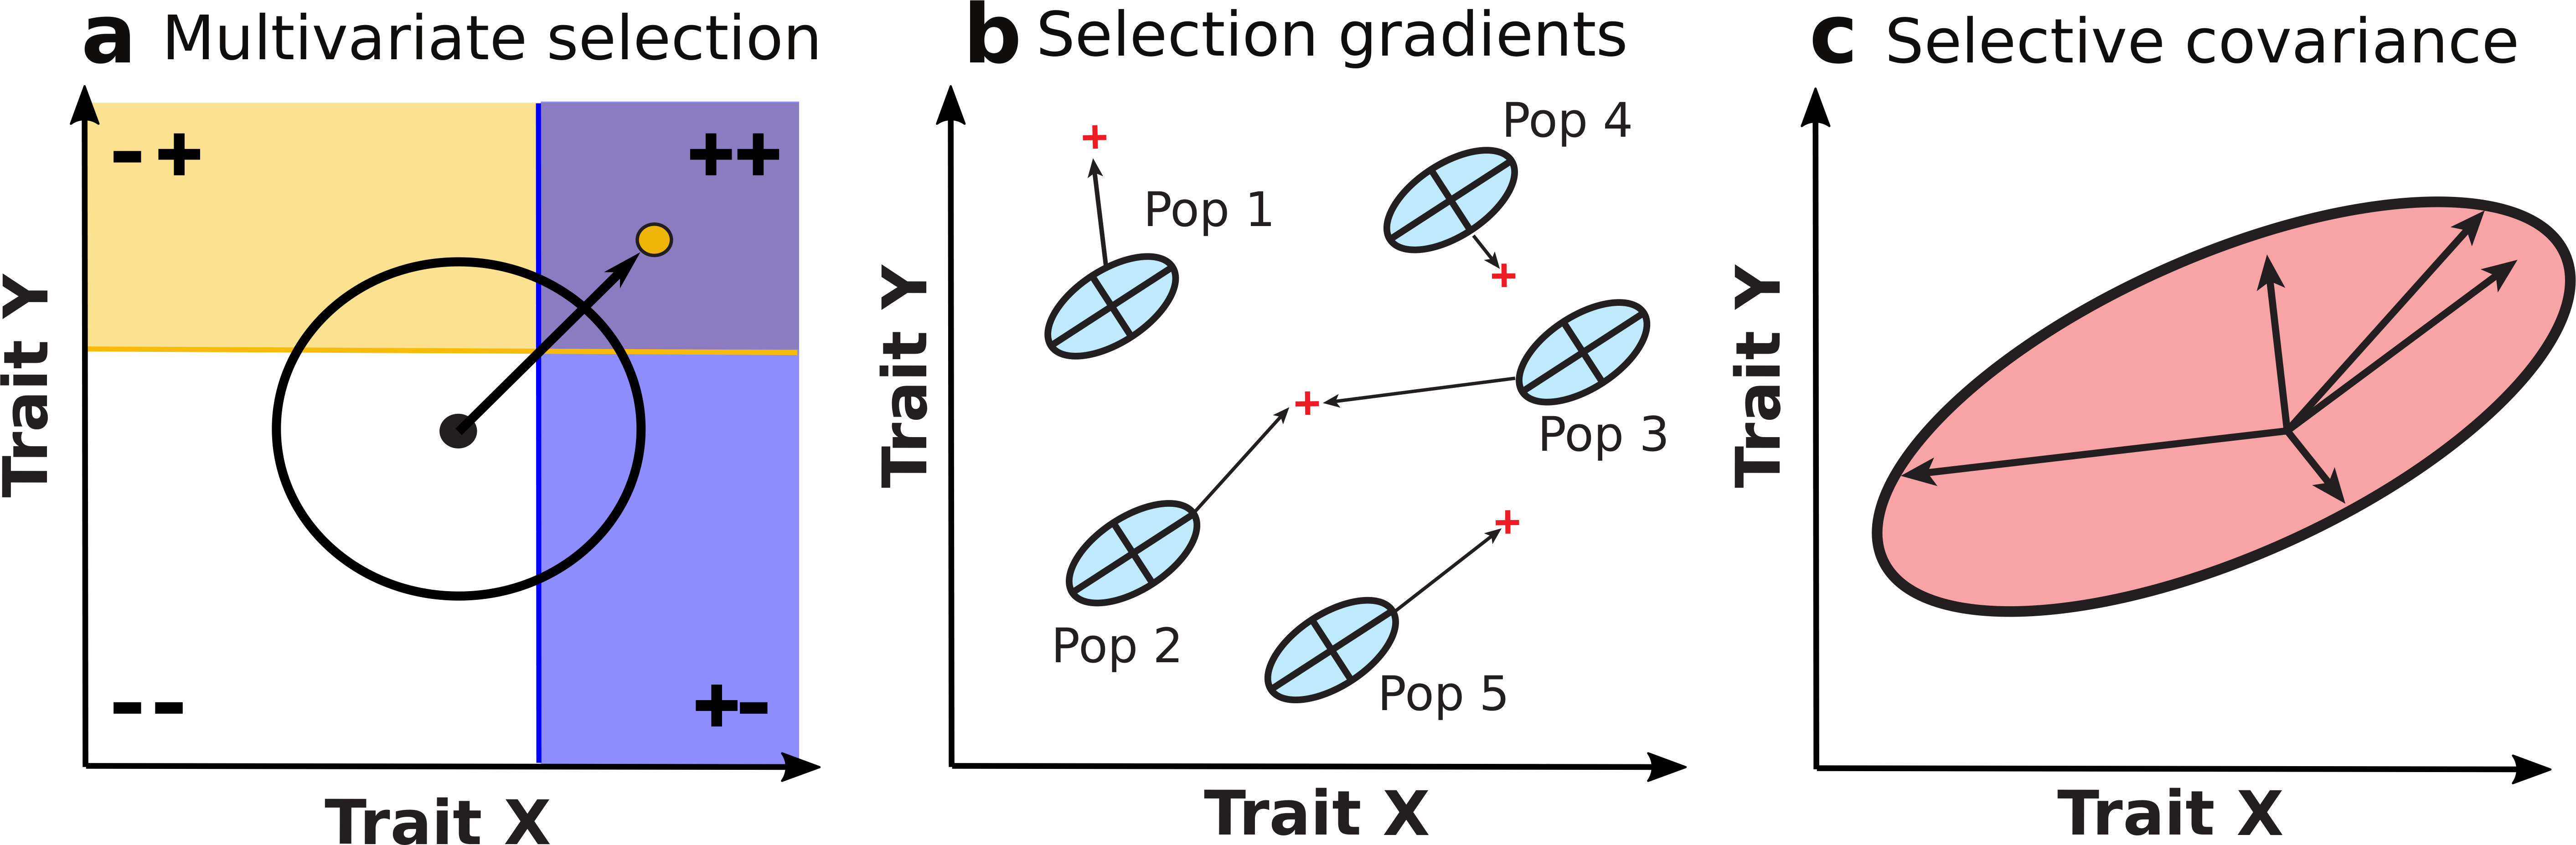
\includegraphics[width=\linewidth]{chapter_annual_review/media/figure4.png}
\caption[Selective covariance]{Traits will evolve together
either because they are inherited together (G-matrix) or because they
are selected together (selective covariance). Panel \emph{a} illustrates
the idea of selective covariance. Traits X and Y are genetically
independent. The black dot indicates the average before selection, and
the plus (+) and minus signs (-)indicate the direction of increase in
fitness for each trait. Thus, selection is favoring the joint increase
of X and Y, and the population will evolve a new average phenotype
(\emph{yellow dot}). The term selective covariance was coined by
\textcite{Felsenstein1988-ql} (see also
\textcite{Zeng1988-or}). If we have evidence that
the G-matrix is relatively stable during macroevolution, the equation V
= GCG captures the covariance of changes in the averages of the species
(V-matrix) in terms of its two potential (non mutually excluding) sources:
inheritance (G-matrix) and selective covariance (C-matrix).
Theoretically, if we have a reasonable estimate of the G-matrix and of
the phylogenetic relationships, we can compute the V-matrix and thus
solve the Zeng-Felsenstein equation to compute C =
G\textsuperscript{-1}VG\textsuperscript{-1}, where C is the covariance
of slopes of log W (e.g., the covariance among the selection gradients
operating upon each species). Panels \emph{b} and \emph{c} illustrate
how to capture the matrix C with selection gradients ($\beta$) on panel
\emph{b} and the selective covariance matrix represented on panel
\emph{c} (\emph{pink ellipse}). Different species are showed by letters
a--e.).}
\label{aree:fig4}
\end{figure}

Comparative approaches establishing a relationship between genetic lines
of least resistance and divergence patterns have other important
limitations. Most significantly, random genetic drift can create an
association between the orientation of the G-matrix and the patterns of
between-species divergence, given stable patterns of genetic
covariation. This association occurs because evolutionary divergence
under drift is expected to be proportional to the ancestral pattern of
variation and covariation among traits
(Fig.~\ref{aree:fig2}) ; therefore, an observed
association between the orientation of the G-matrix and divergence can
be a direct product of neutral evolution. Although most biologists would
agree that morphology is usually under selection, it is useful to
examine the potential consequences of drift and how it relates to
modularity. Simulation work suggests that if genetic drift is the only
operating evolutionary process, modularity patterns would not be stable
and patterns of association would vary widely across closely related
populations or taxa \parencite{Jones2003-jk, Melo2015-bk}. This is
clearly not observed in nature. But what if modularity is maintained by
stabilizing selection and trait means are free to change by genetic
drift? In this situation, divergence among populations would be largest
along directions in which ancestral genetic variation is abundant and
smaller in directions of low ancestral variation \parencite{Arnold2001-lz, Lande1976-xk}. 
There are methods for
distinguishing drift from selection in quantitative traits \parencite{Ackermann2004-ak, Bartoszek2012-mq, Hohenlohe2008-uk, Karhunen2013-dc}, but most of
them are not well suited to high dimensional systems, do not take the
influence of genetic covariation into account, or require a large number
of individuals distributed in a large number of species. For example,
the approach from \textcite{Hohenlohe2008-uk} explicitly models evolution under drift to predict a
probability distribution for the divergence of population averages,
given a phylogeny, the G-matrix, and an estimate of effective population
size. This elegant solution can test whether divergence among groups is
compatible with drift and the current G-matrix, but it can be applied in
full force only with two characters at a time. With few exceptions \parencite{Bartoszek2012-mq, Hohenlohe2008-uk}, most
phylogenetic methods fail to take genetic covariation into account,
thereby limiting our understanding of macroevolution. By modeling
evolution under a univariate Brownian motion model, for example, we
assume that no selection is operating (but see \textcite{Butler2004-jv, Hansen1997-gr})
 and that traits are evolving independently. Some advances have been made in the past decade
\parencite{Bartoszek2012-mq, Cressler2015-xs, Hohenlohe2008-uk}, but we
still lack comparative methods that balance the external aspect of
selection (niche shifts on \textbf{Ornstein-Uhlenbeck} models,
\parencite{Butler2004-jv, Hansen1997-gr} with the populational
consequences of modularity.

\section{Conclusion}

Placing micro- and macroevolution into a common framework is essential
for our understanding of the influence of genetic and developmental
constraints on multivariate evolution. Quantitative genetic theory has
long been interested in the variational properties of organisms, and
recent studies using the conceptual umbrella of modularity have
extrapolated its breadth to include long-term evolutionary change.
Although empirical results led us to discard the notion that variational
patterns are set in stone and act as absolute constraints, they have
also made us abandon the ideas that adaptive landscapes can be
characterized by simple and stable selective peaks or that variational
properties are largely unimportant considerations for evolutionary
change. Embracing the dynamic nature of variational patterns, their
context dependency, as well as their relationships with genetics,
development, and evolution will allow us to bridge these two levels of
the hierarchy in a systematic way. One of the challenges going forward
is the incorporation of mechanistic models of development into models of
how variation emerges and how it influences the shape of population
variation and adaptive landscapes. Another major challenge will be
discriminating the relative contributions of constraints, selection, and
neutral processes in determining the path of multivariate evolution. We
propose that this challenge will be met only when we know more about the
true shape of adaptive landscapes, including the number, height, and
distribution of peaks (see \textcite{Laughlin2015-od, Pfaender2016-eb}),
and when we incorporate modularity into our thinking.

\printbibliography

\end{refsection}